\documentclass[aspectratio=169,11pt,svgnames]{beamer}

\usepackage[english]{babel}
\usepackage{graphicx}
\usepackage{enumitem}
\usepackage{amsmath}
\usepackage{mathtools}
\usepackage{float}
\usepackage{tikz}
\usepackage{tkz-euclide}
\tikzset{point style/.style = {%
  draw = black,
  inner sep = 0pt,
  shape = circle,
  minimum size = 5pt,
  fill = black
 }
}

\usepackage{caption}
\usepackage{subcaption}

% Flowchart stuff

\usepackage{pgfopts}
\usepackage{xcolor}
\usepackage{tcolorbox}

\usetheme[
 titlestyle=style2,
 titleformat=smallcaps,
 sectionstyle=plain,
 slidestyle=cyber,
 headingcolor=theme,
 block=transparent
]{trigon}

\title{Polygons}
\date{\today}
\author{Adam Klepáč}
\institute[GEVO]{Gymnázium Evolution Jižní Město}
\biglogo[width=.2\textwidth]{logo}
\smalllogo[width=.1\textwidth]{logo}
\titlegraphic{
\includegraphics[height=\paperheight]{title.jpg}}

\def\subsectionname{}

% enumerate global settings
\setlist[enumerate,1]{label=\arabic*.}
\setlist[enumerate,2]{label=\alph*)}

% custom colors %
\definecolor{PolygonYellow}{HTML}{f6e01a}
\definecolor{PolygonCyan}{HTML}{11cdef}
\definecolor{PolygonOrange}{HTML}{b25c10}
\definecolor{PolygonBlue}{HTML}{0a2a66}
\colorlet{tPrim}{PolygonBlue}
\colorlet{tTheme}{PolygonYellow}
\colorlet{tSec}{PolygonCyan}
\colorlet{tAccent}{PolygonCyan}

\tcbset{
 boxsep=7pt,
 fonttitle=\sc,
 colframe=tGreyBg,
 colframe=tPrim,
 boxrule=1pt
}

\begin{document}
\titleframe

\begin{frame}
 \frametitle{Contents}
 \tableofcontents
\end{frame}

\section{General Polygons}
\label{sec:general-polygons}

\begin{frame}
 \frametitle{General Polygons -- Def~\hspace{-.4ex}inition}
 \begin{tcolorbox}[title=Polygon]
  A \alert{polygon} is a closed 2D shape made of only segments.
 \end{tcolorbox}
 \begin{itemize}
  \item<2-> The endpoints of those segments are called \alert{vertices}.
  \item<3-> The segments themselves are called \alert{edges}.
 \end{itemize}
\end{frame}

\begin{frame}
 \frametitle{General Polygons -- Examples}
 \begin{figure}[H]
  \centering
  \begin{subfigure}[b]{.23\textwidth}
   \centering
   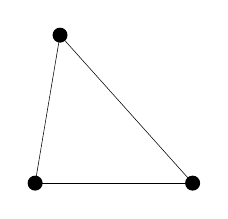
\begin{tikzpicture}
    \tkzDefPoint(0:1){A}
    \tkzDefPoint(110:2){B}
    \tkzDefPoint(180:1){C}

    \tkzDrawPoints(A,B,C);
    \tkzDrawSegments(A,B B,C C,A);
   \end{tikzpicture}
   \caption*{Triangle}
  \end{subfigure}
  \begin{subfigure}[b]{.23\textwidth}
   \centering
   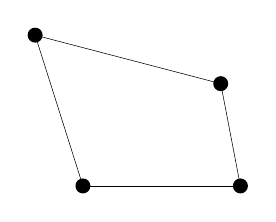
\begin{tikzpicture}
    \tkzDefPoint(0:1){A}
    \tkzDefPoint(60:1.5){B}
    \tkzDefPoint(130:2.5){C}
    \tkzDefPoint(180:1){D}

    \tkzDrawPoints(A,B,C, D);
    \tkzDrawSegments(A,B B,C C,D D,A);
   \end{tikzpicture}
   \caption*{Quadrilateral}
  \end{subfigure}
  \begin{subfigure}[b]{.23\textwidth}
   \centering
   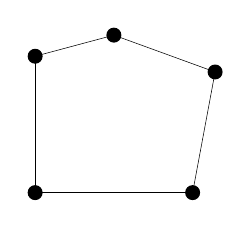
\begin{tikzpicture}
    \tkzDefPoint(0:1){A}
    \tkzDefPoint(50:2){B}
    \tkzDefPoint(90:2){C}
    \tkzDefPoint(120:2){D}
    \tkzDefPoint(180:1){E}

    \tkzDrawPoints(A,B,C,D,E);
    \tkzDrawSegments(A,B B,C C,D D,E E,A);
   \end{tikzpicture}
   \caption*{Pentagon}
  \end{subfigure}
  \begin{subfigure}[b]{.27\textwidth}
   \centering
   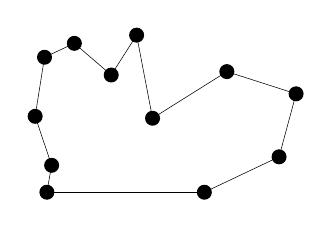
\begin{tikzpicture}
    \tkzDefPoint(0:1){A}
    \tkzDefPoint(13:2){B}
    \tkzDefPoint(30:2.5){C}
    \tkzDefPoint(50:2){D}
    \tkzDefPoint(70:1){E}
    \tkzDefPoint(86:2){F}
    \tkzDefPoint(97:1.5){G}
    \tkzDefPoint(109:2){H}
    \tkzDefPoint(121:2){I}
    \tkzDefPoint(140:1.5){J}
    \tkzDefPoint(160:1){K}
    \tkzDefPoint(180:1){L}

    \tkzDrawPoints(A,B,C,D,E,F,G,H,I,J,K,L);
    \tkzDrawSegments(A,B B,C C,D D,E E,F F,G G,H H,I I,J J,K K,L L,A);
   \end{tikzpicture}
   \caption*{Dodecagon}
  \end{subfigure}
 \end{figure}
 \begin{itemize}
  \item <2-> A polygon with $n \in \mathbb{N}$ sides is called an $n$-gon.
  \item <3-> For example a polygon with 123456 sides is called a $123456$-gon or
   decadismyriatrischilliatetrahectapentacontakaihexagon.
 \end{itemize} 
\end{frame}

\begin{frame}
 \frametitle{General Polygons -- Counterexamples}
 \begin{figure}[H]
  \centering
  \begin{subfigure}[b]{.33\textwidth}
   \centering
   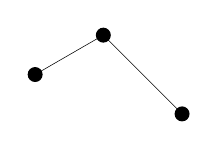
\begin{tikzpicture}
    \tkzDefPoint(0:1){A}
    \tkzDefPoint(90:1){B}
    \tkzDefPoint(150:1){C}

    \tkzDrawPoints(A,B,C);
    \tkzDrawSegments(A,B B,C);
   \end{tikzpicture}
   \caption*{Not closed}
  \end{subfigure}
  \begin{subfigure}[b]{.33\textwidth}
   \centering
   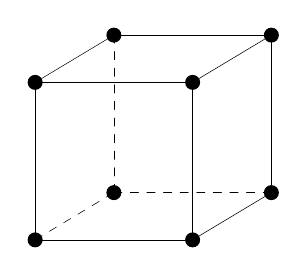
\begin{tikzpicture}[scale=2]
    \tkzDefPoint(0,0){A1}
    \tkzDefPoint(0,1){B1}
    \tkzDefPoint(1,1){C1}
    \tkzDefPoint(1,0){D1}

    \tkzDefPoint(0.5,0.3){A2}
    \tkzDefPoint(0.5,1.3){B2}
    \tkzDefPoint(1.5,1.3){C2}
    \tkzDefPoint(1.5,0.3){D2}
    \tkzDrawPoints(A1,B1,C1,D1,A2,B2,C2,D2)

    \tkzDrawSegments(A1,B1 B1,C1 C1,D1 D1,A1 B2,C2 C2,D2 B1,B2 C1,C2 D1,D2)
    \tkzDrawSegments[dashed](A2,B2 D2,A2 A1,A2)
   \end{tikzpicture}
   \caption*{3D}
  \end{subfigure}
  \begin{subfigure}[b]{.33\textwidth}
   \centering
   \begin{tikzpicture}
    \tkzDefPoint(0:1){A}
    \tkzDefPoint(180:1){B}
    \tkzDefPoint(90:1){P}

    \tkzDrawPoints(A,B)
    \tkzDrawArc(P,A)(B)
    \tkzDrawSegment(A,B)
   \end{tikzpicture}
   \caption*{Not straight}
  \end{subfigure}
 \end{figure}
\end{frame}

\begin{frame}
 \frametitle{General Polygons -- Convexity}
 \begin{tcolorbox}[title=Convex Polygon]
  A polygon is called \alert{convex} if it has no internal angle greater than
  180$^{\circ}$.
 \end{tcolorbox}
 \pause
 \begin{figure}[H]
  \centering
  \begin{subfigure}[b]{.45\textwidth}
   \centering
   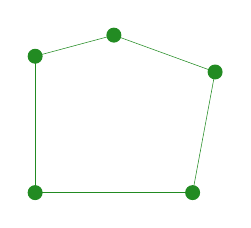
\begin{tikzpicture}
    \tkzDefPoint(0:1){A}
    \tkzDefPoint(50:2){B}
    \tkzDefPoint(90:2){C}
    \tkzDefPoint(120:2){D}
    \tkzDefPoint(180:1){E}

    \tkzDrawPoints[color=ForestGreen](A,B,C,D,E);
    \tkzDrawSegments[color=ForestGreen](A,B B,C C,D D,E E,A);
   \end{tikzpicture}
   \caption*{\textcolor{ForestGreen}{Convex}}
  \end{subfigure}
  \begin{subfigure}[b]{.45\textwidth}
   \centering
   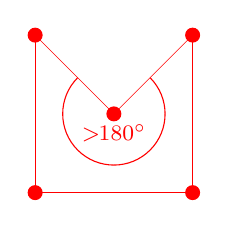
\begin{tikzpicture}
    \tkzDefPoint(0,0){A}
    \tkzDefPoint(2,0){B}
    \tkzDefPoint(2,2){C}
    \tkzDefPoint(1,1){D}
    \tkzDefPoint(0,2){E}

    \tkzDrawPoints[color=Red](A,B,C,D,E)
    \tkzDrawSegments[color=Red](A,B B,C C,D D,E E,A)

    \tkzMarkAngle[color=Red,size=0.65](E,D,C)
    \tkzLabelAngle[color=Red,pos=0.25](E,D,C){\footnotesize $>\!\!180^{ \circ}$}
   \end{tikzpicture}
   \caption*{\textcolor{Red}{NOT convex}}
  \end{subfigure}
 \end{figure}
\end{frame}

\section{Convex Polygons}
\label{sec:convex-polygons}

\begin{frame}
 \frametitle{Convex Polygons -- Diagonals}
 \begin{tcolorbox}[title=Diagonal in A Convex Polygon]
  A \alert{diagonal} is a segment connecting two non-adjacent vertices.
 \end{tcolorbox}
 \begin{figure}[H]
  \centering
  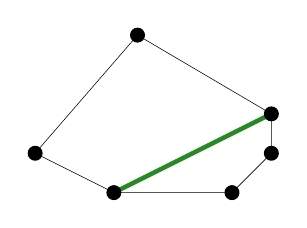
\begin{tikzpicture}
   \tkzDefPoint(0,0){A}
   \tkzDefPoint(-1,0.5){B}
   \tkzDefPoint(0.3,2){C}
   \tkzDefPoint(2,1){D}
   \tkzDefPoint(2,0.5){E}
   \tkzDefPoint(1.5,0){F}
   
   \tkzDrawPolygon(A,B,C,D,E,F)
   \tkzDrawSegment[color=ForestGreen,ultra thick](A,D)
   \tkzDrawPoints(A,B,C,D,E,F)
  \end{tikzpicture}
  \caption*{\textcolor{ForestGreen}{Diagonal} in a convex hexagon.}
 \end{figure}
\end{frame}

\end{document}
